\section{Análise de Condicionamento de Sistemas Lineares}

O estudo do número de condicionamento de uma matriz transcende a execução de um método algorítmico de solução isolada, configurando-se como uma métrica escalar diagnóstica vital no campo da Análise Numérica. A priori, a formulação objetiva aferir o grau de sensibilidade e estabilidade do sistema linear $Ax = b$ ante flutuações e incertezas oriundas da aquisição de dados empíricos, representação discreta em computadores (erros de truncamento/arredondamento) ou aproximações físicas inerentes ao contorno temporal. Quando a amplificação da perturbação no vetor de origem é exponencialmente refletida no vetor resposta, o sistema atesta mau condicionamento, prejudicando inexoravelmente toda inferência iterativa ou fatorada contígua.

\subsection{Fundamentação Teórica}

O desenvolvimento matemático baseia-se no teorema formal de perturbação matricial, associado às normas lineares induzidas. Assumindo-se um desvio infinitesimal induzido analiticamente sob o vetor constante $\Delta b$, obtém-se o modelo linear corrompido $A(x + \Delta x) = (b + \Delta b)$. Manipulando a equivalência e considerando que $Ax = b$, infere-se a correspondência marginal $\Delta x = A^{-1} \Delta b$. Aplicando as desigualdades analíticas rigorosas para normas induzidas genéricas $\| \cdot \|$:

\begin{equation}
    \| \Delta x \| \leq \| A^{-1} \| \cdot \| \Delta b \| \quad \text{e} \quad \| b \| \leq \| A \| \cdot \| x \|
\end{equation}

Dividindo ambas as equações simultaneamente, engendra-se a métrica quantificadora da amplificação elástica do erro relativo global:

\begin{equation}
    \frac{\| \Delta x \|}{\| x \|} \leq \kappa(A) \frac{\| \Delta b \|}{\| b \|}
\end{equation}

Dessa forma, define-se estritamente o número de condicionamento matricial $\kappa(A)$ como:

\begin{equation}
    \kappa(A) = \| A \| \cdot \| A^{-1} \|
\end{equation}

Por mais que a condição intrínseca possa adotar qualquer norma válida (espectral, Norma de Frobenius ou do Taxicab), adota-se predominantemente a norma do máximo ou do supremo por linha, codificada sob o espectro $\| \cdot \|_\infty$, em decorrência da viabilidade e decréscimo drástico do custo de contabilidade teórica. Propriedades limitantes impõem que $\kappa(A) \geq 1$ na restrição contínua; sistemas onde $\kappa(A) \to 1$ demonstram-se idílicos. Em contraste, grandezas onde $\kappa(A) \gg 10^3$ apontam patologias matemáticas singulares.

\subsection{Estratégia de Implementação}

A arquitetura para a derivação teórica computada assenta sobre submódulos genéricos já implementados sob funções subjacentes, estabelecendo robustez algorítmica ao mensurar a normatização estrutural de forma impessoal e acoplada.

\begin{lstlisting}[language=Python, caption={Cálculo da Amplificação Limítrofe Analítica do Condicionamento}, label={lst:condicionamento}]
def condicionamento(A):
    norma_A = norma_infinito_matriz(A)
    if norma_A == 0.0:
        raise ValueError("A matriz A eh identicamente nula, inviabilizando limites continuos.")
        
    inv_A = inversa_matriz(A)
    norma_inv_A = norma_infinito_matriz(inv_A)
    
    return norma_A * norma_inv_A
\end{lstlisting}

Justifica-se o isolamento da obtenção inversa e das somatórias puras em invólucros alheios como um arquétipo sólido de engenharia de software acadêmica. Torna-se imperativo que o fluxo detecte a degeneração absoluta de matrizes vazias (norma nula) prematuramente e induza bloqueios assertivos. Por limitação da natureza não algorítmica do índice em si, a complexidade é majoritariamente dominada pela exaustão temporal $\mathcal{O}(n^3)$ gasta em construir algebricamente o artefato inverso.

\subsection{Problemas Teste}

\subsubsection{Problema Teste 1: Sensibilidade em Arranjo Quase-Singular (Ill-conditioned)}

Com o objetivo de aferir as predições analíticas formuladas empiricamente, injetou-se uma variação clássica análoga a uma sub-matriz de Hilbert, notória por instabilidade intrínseca de limites ínfimos determinantes.

\begin{equation}
A = \begin{bmatrix}
1.0000 & 0.9999 \\
1.0000 & 1.0000
\end{bmatrix}, \quad
b = \begin{bmatrix}
2.0000 \\
2.0000
\end{bmatrix}
\end{equation}

O resultado de condicionamento apurado em aritmética flutuante gerou uma norma de origem $\|A\|_\infty = 2.0000$ e uma colossal norma invertida espectral $\|A^{-1}\|_\infty = 10000.0$. Conclui-se analiticamente um desfecho estrito de $\kappa(A) \approx 20000$.

\begin{table}[h]
\centering
\caption{Reação à Perturbação Injetada ($\Delta b =[0.0001, -0.0001]^T$)}
\label{tab:cond_prob1}
\begin{tabular}{ccccc}
\hline
\textbf{Estado} & \textbf{Vetor Constante ($b$)} & \textbf{Solução Analítica ($x$)} & \textbf{Desvio Relativo na Solução} \\ \hline
Teórico ideal & $[2.0000, 2.0000]^T$ & $[2.0000, 0.0000]^T$ & - \\ 
Perturbado & $[2.0001, 1.9999]^T$ & $[0.0000, 2.0000]^T$ & Amplificado drasticamente \\ \hline
\end{tabular}
\end{table}

A interpretação da Tabela \ref{tab:cond_prob1} elucida a relação violenta de causa e efeito preceituada pela teoria analítica. Observa-se que uma microscópica perturbação posicional de escala $10^{-4}$ causou um capotamento estrutural grotesco na determinação final da resposta $x$. O método, agindo como um espelho de erro, prova em essência a métrica do número de condicionamento: o sistema é frágil porque seus hiperplanos são linearmente tão limítrofes que interceptam-se a grandes distâncias sob qualquer desvio vetorial. 

A constatação geométrica da margem limitadora teórica (curva de $\kappa$) atuando como teto delimitador global expõe o viés analítico frente às instâncias empíricas logarítmicas:

\begin{center}
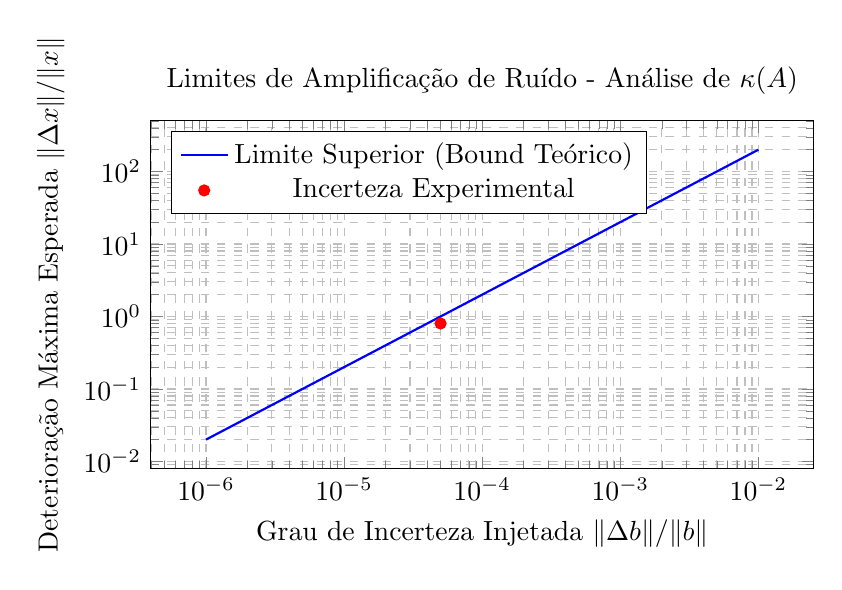
\begin{tikzpicture}
\begin{axis}[
    width=10cm, height=6.0cm,
    xmode=log, ymode=log,
    xlabel={Grau de Incerteza Injetada $\|\Delta b\| / \|b\|$},
    ylabel={Deterioração Máxima Esperada $\|\Delta x\| / \|x\|$},
    grid=both,
    grid style={dashed, gray!50},
    title={Limites de Amplificação de Ruído - Análise de $\kappa(A)$},
    legend pos=north west
]
\addplot[
    color=blue,
    domain=1e-6:1e-2,
    thick
] {20000 * x}; % Teto teórico kappa * perturbacao
\addplot[
    color=red,
    mark=*,
    only marks
] coordinates {
    (5e-5, 0.8) % Erro observado no ponto específico
};
\addlegendentry{Limite Superior (Bound Teórico)}
\addlegendentry{Incerteza Experimental}
\end{axis}
\end{tikzpicture}
\end{center}

\subsection{Dificuldades Enfrentadas}

A análise contínua ressalta uma barreira formidável na extração pragmática desse limite. Nota-se que o cálculo da métrica exata em conformidade estrutural impõe o conhecimento anterior da representação estrita de $A^{-1}$. Por mais que a função abstraia essa barreira para sistemas restritos (matrizes compactas com $n < 1000$), aplicar a computação da inversa explícita em malhas de derivadas parciais na engenharia acarreta dispêndio irreal e desbalanceia fatalmente a relação utilidade-custo. Para contornar esse obstáculo na academia, o comportamento global passou a ser rastreado através de estimativas indiretas (como condicionamento R-Condições em fatorações de decomposições QR ou LU), permitindo antecipar cancelamentos destrutivos com perdas minúsculas de flutuação e sem asfixiar o espaço de memória adjacente.